\documentclass[11pt]{article}
  \renewcommand{\baselinestretch}{1.05}
  \usepackage{amsmath,amsthm,verbatim,amssymb,amsfonts,amscd,graphicx}
  \usepackage{graphics}
  \usepackage{url}
  \usepackage[utf8]{inputenc}
  \graphicspath{{images/}}
  \topmargin0.0cm
  \headheight0.0cm
  \headsep0.0cm
  \oddsidemargin0.0cm
  \textheight23.0cm
  \textwidth16.5cm
  \footskip1.0cm
  \theoremstyle{plain}
  \newtheorem{theorem}{Theorem}
  \newtheorem{corollary}{Corollary}
  \newtheorem{lemma}{Lemma}
  \newtheorem{proposition}{Proposition}
  \newtheorem*{surfacecor}{Corollary 1}
  \newtheorem{conjecture}{Conjecture}
  \newtheorem{question}{Question}
  \theoremstyle{definition}
  \newtheorem{definition}{Definition}
  \renewcommand{\figurename}{Kuva}

   \begin{document}

  \title{Neuroverkot}
  \author{Teemu Sarapisto}
  \maketitle


  %Neuroverkot saivat alkunsa jo 40-luvulla, mutta vasta 2006 tarvittavat palaset niiden läpimurtoon saatiin kasaan (katso millaisella kielellä papereita yleensä aloitetaan).

  %Tietokoneiden suorituskyvyn kasvamisen, suurien määrien luokiteltua dataa löytymisen ja sopivien algoritmien kuten backpropagationin  (suomenna) yleistymisen myötä neuroverkot alkoivat noin 2006 alkaen ratkaista ongelmia joihin ei muilla lähestymistavoilla oltu aikaisemmin pystytty. suurta suosiota, oltuaan jo aikaisemmin sekä 40-60 luvuilla, että 80-95 vuosina jo vahvasti pinnalla.

  %Neuroverkot ovat jo pari kertaa olleet pinnalla, mutta niiden todelliseen läpilyömiseen tarvitut osaset löytyivät vasta 2006, kun suuret määrät luokiteltua dataa tuli helposti saataville, ja näytönohjainten tietokoneiden suorituskyvyn kasvettua mm. näytonohjainten hyödyntämisen kautta tarpeeksi suurelle tasolle jotta neuroverkkojen tehokas hyödyntäminen tuli mahdolliseksi. Myös back-propagation.
  Viimeisen hieman yli kymmenen vuoden aikana voidaan sanoa keinotekoisten neuroverkkojen ja syväoppimisen tehneen läpimurron. Syväoppimisen voidaan katsoa syntyneen jo 40-luvulla, mutta laajamittaiseen sovelluskäyttöön se on tullut vasta viime vuosina, kun sekä riittävä määrä luokiteltua dataa, että riittävästi prosessointitehoa on tullut helposti saataville. Myös algoritmipuolella tapahtuneet edistykset ovat edesauttaneet läpimurtoa. Aikaisemmin koneoppimisen alalla haasteelliseksi osoittautuneissa sovelluskohteissa kuten kuvien sekä puheen sisällön tunnistamisessa keinotekoiset neuroverkot ovat osoittautuneet toistaiseksi ylivoimaisesti parhaiten toimiviksi ratkaisuiksi.

  \section{Neuroverkkojen rakenne}
  \subsection{Keinotekoinen neuroni}


    Biologisista vaikuttimistaan huolimatta keinotekoiset neuronit ovat käytännössä Kaavan \ref{eq:neuroni} muotoisia matemaattisia funktioita.

    \begin{equation}
      \label{eq:neuroni}
      \Sigma w_i x_i \mapsto f(\Sigma w_i x_i + b)
    \end{equation}

    Yleisessä muodossaan neuroni ottaa vastaan yhden tai useampia syötteitä $x_1$, $x_2$, ..., $x_n$, joista kullekin on asetettu jokin painoarvo $w_i$. Syötteiden ja painotuksien tulojen summa $\Sigma x_i w_i$ annetaan parametrina aktivaatiofunktiolle $f$ ja tämän funktion arvo toimii neuronin lopullisena ulostuloarvona.

    Toisinaan käytetään myös taipumusvakiota (bias) $b$, joka lisätään syötteiden ja painotuksien tulojen summaan.


    %You can think of the bias as a measure of how easy it is to get the perceptron to output a 1. Or to put it in more biological terms, the bias is a measure of how easy it is to get the perceptron to fire

    Ensimmäinen tällainen neuroni, perseptroni, kehitettiin 50-luvulla. Sen syötteet ja ulostuloarvot ovat binäärisiä ja aktivaatiofunktiona toimii Kaavan \ref{eq:perceptron} mukainen funktio.

    \begin{equation}
      \label{eq:perceptron}
      ulostuloarvo
      \begin{cases}
        0\; jos \; \Sigma x_i w_i + b \leq 0 \\
        1\; jos \; \Sigma x_i w_i + b > 0 \\
      \end{cases}
    \end{equation}

    Yksittäisen neuronin tasolla neuronien oppiminen tapahtuu syötteiden painotuksien ja taipumusarvon muuttumisen kautta. Perseptroneja käytettäessä törmätään kuitenkin usein ongelmaan, jossa yksi pieni muutos painotuksissa tai taipumusarvossa johtaa ulostuloarvon vaihtumiseen, joka saattaa aiheuttaa suuria muutoksia ulostuloarvoissa myös koko neuroverkon tasolla. Usein halutaan hienovaraisempia muutoksia ja siksi usein käytetään neuroneita joiden syöte- ja paluuarvot voivat olla myös mitä vain reaalilukuja nollan ja yhden väliltä. Esimerkiksi yksi tällainen laajalti käytössä oleva neuroni on sigmoidinen neuroni, jonka aktivaatiofunktiona toimii sigmoidinen funktio.

  %kappaleessa 3 rojanista hyvää juttua \cite{Rojas96}

  %http://neuralnetworksanddeeplearning.com/chap1.html keksi parempi lähde
  % oliko varmasti 50-luvulla?

  \subsection{Keinotekoisten neuroverkkojen rakenne}

  \begin{figure}[h]
  \label{pic:neuralnet}
  \centering
  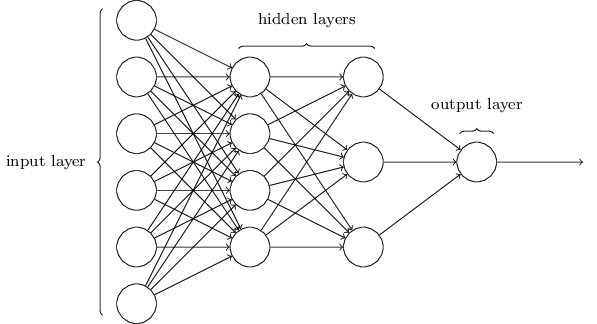
\includegraphics[scale=0.5]{basic-neuralnet}
  \caption{http://neuralnetworksanddeeplearning.com/chap1.html}
  \end{figure}

  Yksinkertaisimman verkkorakenteen omaavat eteenpäinsyöttävät neuroverkot muodostetaan tasoittain, jossa jokaisen verkon tason neuronit saavat syötteenään niitä edeltävän tason neuroneiden ulostuloarvot. Poikkeuksena ensimmäinen taso (kuvassa vasemmanpuoleisimpana), joihin verkon syöte koodataan. Esimerkiksi haluttaessa syöttää 64x64 kuva neuroverkolle, voidaan syötekerroksena käyttää 64x64 neuronin kerrosta, johon kuvan pikselien väriarvot koodataan.

  Vaikka syväoppimista voidaan harjoittaa myös muutoin kuin keinotekoisilla neuroverkoilla, neuroverkkojen tapauksessa termillä viitataan neuroverkkojen piilokerroksiin ja niiden määrään. Kasvattamalla neuroverkkotasojen sekä tasoissa olevien neuronien määrää, neuroverkoilla voidaan mallintaa entistä monimutkaisempia funktioita.

  \section{Neuroverkkojen oppiminen}
  Neuroverkkoa opetettaessa tavoitteena on minimoida neuroverkon tekemä virhe sen approksimoidessa jotakin funktiota. Tämän virheen määrää arvioidaan virhefunktion (error function) avulla. Neuroverkon laskiessa ulostuloarvon jollekkin syötteelle, tapahtuu eteenpäinkulkeutumista (forward-propagation). Taaksepäinkulkeutumiseksi (back-propagation) kutsutaan algoritmiä jonka avulla jollekkin neuroverkon painoille määritellylle virhefunktiolle lasketaan gradientti, jonka perusteella neuroverkon approksimoinnin virhettä voidaan lähteä pienentämään gradientin laskeutumismenetelmää käyttäen.

  Suuri haaste neuroverkkojen opetuksessa on ylisovitus (overfitting) jossa neuroverkon virhefunktion arvo on harjoitusdatalla saatu erittäin pieneksi, mutta uuden datan kanssa virhefunktio antaa suuria arvoja. Tällöin neuroverkon oppima malli vastaa harjoitusdataa liian tarkkaan, eikä enää suoriudu yleisestä tapauksesta toivotulla tavalla. Ylisovitusta korjaamaan on kehitetty metodeja kuten esimerkiksi neuroniyksikköjen pudotus (dropout) jossa opetusvaiheessa yksittäisiä neuroneita poistetaan käytöstä, joka estää yksittäisiä neuroneita naapureineen erikoistumatta tiettyyn datan ominaisuuteen liian tarkasti.

  Neuroverkkojen opetuksessa olennaisessa osassa on myös verkon alkuperäisten painotuksien valitseminen sopivalla tavalla.

  \nocite{*}

  \renewcommand{\refname}{Lähteet}
  \bibliographystyle{ieeetr}
  \bibliography{test}

  \end{document}